\documentclass{article}
\usepackage[margin=1in]{geometry}
\usepackage[utf8]{inputenc}
\usepackage[T1]{fontenc}
\usepackage{hyperref}
\usepackage{url}
\usepackage{booktabs}
\usepackage{amsfonts}
\usepackage{amsmath}
\usepackage{amssymb}
\usepackage{graphicx}

\title{Supplement: Verifier-Guided Constraint Projection}
\author{Anonymous Authors}

\begin{document}

\maketitle

\appendix

\section{Implementation details of the verifier}
\label{sec:supp-verifier}

The pairwise overlap matrix $A \in \mathbb{R}^{N \times N}$ is computed as follows (PyTorch pseudocode):
\begin{verbatim}
  # centers: (N, 2), sizes: (N, 2)
  cx, cy = centers[:, 0], centers[:, 1]
  sw, sh = sizes[:, 0], sizes[:, 1]

  # pairwise AABB
  ovx = torch.clamp_min(
      torch.minimum(cx[:, None] + sw[:, None]/2, cx[None, :] + sw[None, :]/2) -
      torch.maximum(cx[:, None] - sw[:, None]/2, cx[None, :] - sw[None, :]/2),
      0,
  )
  ovy = torch.clamp_min(
      torch.minimum(cy[:, None] + sh[:, None]/2, cy[None, :] + sh[None, :]/2) -
      torch.maximum(cy[:, None] - sh[:, None]/2, cy[None, :] - sh[None, :]/2),
      0,
  )
  A = ovx * ovy
  A.fill_diagonal_(0)  # exclude self-overlap
\end{verbatim}

Boundary violation for each macro along axis $a \in \{x,y\}$ and edge $e \in \{-,+\}$:
\begin{equation}
  b_i^{a,-} = \max(0, s_i^a/2 - c_i^a),
  \qquad b_i^{a,+} = \max(0, c_i^a + s_i^a/2 - W_a),
\end{equation}
with $b_i = \sum_a (b_i^{a,-} + b_i^{a,+})$.

\section{Neural repair operator: full training details}
\label{sec:supp-neural}

\paragraph{Architecture.} 3-layer GATv2 (heads=4, hidden=128), scale-invariant input normalization (centers and severity are divided by $\max(W, H)$). Node features: $[\mathrm{severity}, \mathrm{boundary}, \mathrm{n\_overlappers}, s^w, s^h]$. Edge features: 4-dim pin offsets (from ChipDiffusion's edge\_attr).

\paragraph{Loss.} L2 on the predicted displacement against a target defined by the variant (see below).

\paragraph{Variants.}
\begin{itemize}
\item \textbf{Synthetic teacher}: hand-crafted operator applied to synthetic placements from ChipDiffusion's data generator. 2500 training graphs, 200 val.
\item \textbf{Real teacher}: hand-crafted operator on diffusion-sampled ISPD2005 placements (3 samples per circuit × 1--3 circuits = 3--9 samples depending on seed).
\item \textbf{Data augmentation}: per-sample $\times 50$ random Gaussian perturbations of the baseline.
\item \textbf{Trajectory distillation}: $(x_k, x_{k+1})$ pairs from every step of the hand-crafted operator; 30 steps $\times$ 3 samples = 90 pairs.
\item \textbf{Ground-truth target}: ISPD2005 industrial \texttt{.pl} placements as target.
\item \textbf{Residual learning}: train to predict $x_{GT} - x_{\text{hand}}$ after hand-crafted convergence; apply as residual scale $s \in \{0.01, 0.05, 0.1, 0.2\}$.
\end{itemize}

\paragraph{Training.} Adam, lr $10^{-3}$, 100 epochs, batch 1 (per-graph), early stop on val loss.

\paragraph{Findings.} Best val loss was 0.0037 (trajectory distillation), but at inference on ISPD2005 the best variant (residual $s=0.1$) improved violations on 1 of 6 circuits while degrading HPWL. Detailed per-circuit results are available in \texttt{results/neural\_vsr/eval\_*.json}.

\section{Extended Pareto results}
\label{sec:supp-pareto}

Full per-seed per-$\lambda$ results are in \texttt{results/ispd2005/pareto\_3seed\_6w.json}. The 3-seed standard deviation for $\Delta$viol is $< 4\%$ on 5 of 6 circuits and $< 8\%$ on adaptec2. The standard deviation for $\Delta$HPWL is circuit-dependent: under 15\% for adaptec1--4 and bigblue3, and up to 20\% on bigblue1 where baseline HPWL is very small and therefore percent-changes are noisier.

\section{Convergence curves}
\label{sec:supp-convergence}

Figure~\ref{fig:supp-convergence} (attached) shows per-iteration $(v_t, h_t)$ trajectories for $T=300$ iterations on adaptec1 and bigblue1 at $\lambda=2$. Violations decrease near-monotonically; HPWL changes non-monotonically in the first $\sim 30$ iterations (as the repulsive force initially pushes connected macros apart) before the attractive term pulls them back. The plateau is reached by $T \approx 100$, consistent with the num\_steps ablation.

\begin{figure}[h]
\centering
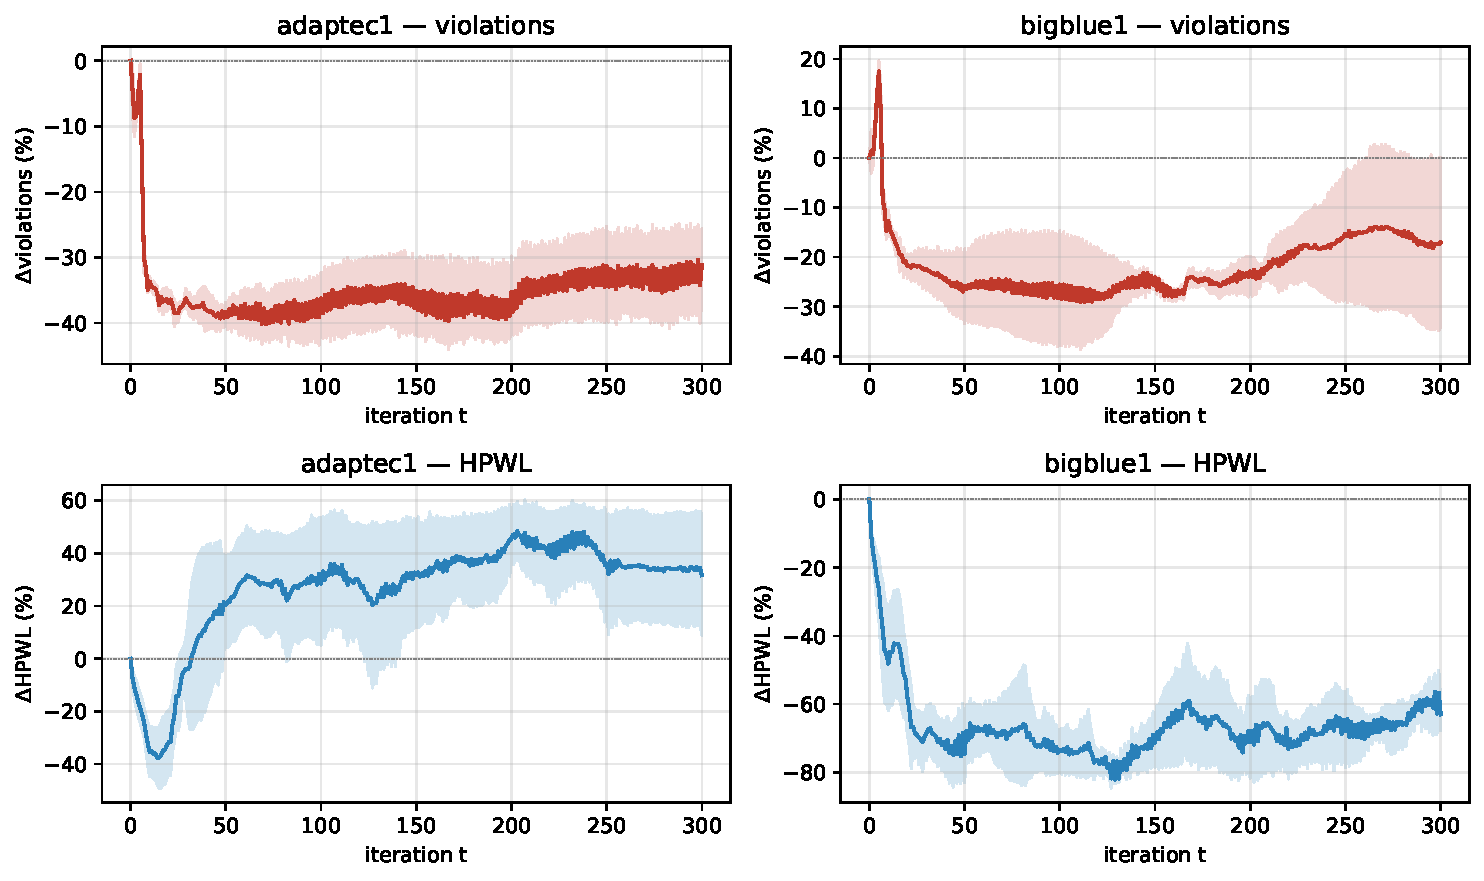
\includegraphics[width=0.85\linewidth]{figures/fig7_convergence.pdf}
\caption{Per-iteration convergence for VSR on adaptec1 and bigblue1, 3 seeds each. Top row: violations vs.\ iteration. Bottom row: HPWL vs.\ iteration. Shaded band = seed std.}
\label{fig:supp-convergence}
\end{figure}

\section{Full ablations and extra figures}
\label{sec:supp-ablations}

\paragraph{Number of steps $T$ (Fig.~\ref{fig:supp-numsteps}).} Violations plateau near $T=100$; going to $T=500$ gains $<2\%$ on all circuits and HPWL is stable.

\paragraph{Step size $\eta$ (Fig.~\ref{fig:supp-stepsize}).} $\eta=0.3$ (default) is the robust middle ground. $\eta=1.0$ gains marginal violation reduction at higher HPWL variance.

\paragraph{Selective vs.\ global (Tab.~\ref{tab:supp-selective}).} Identical on ISPD2005 raw drafts because every macro violates.

\paragraph{Intra-sampling start timestep (Fig.~\ref{fig:supp-timestep}).}
The full 6-circuit, 5-timestep sweep shows that the intra-sampling
HPWL benefit is monotonically stronger with larger $t_{\text{start}}$
on the largest circuit: bigblue3 reaches $-34.5\%$ HPWL at
$t_{\text{start}}=0.5$, $-37.8\%$ at $t_{\text{start}}=0.7$ (median across 3
seeds).  On adaptec3 the curve is shallower ($-12.6\%$ at $t=0.1$, decaying to
$-5.1\%$ at $t=0.7$).  On the smaller circuits (adaptec1, adaptec2,
bigblue1) the absolute HPWL change is within $\pm 5\%$ across all $t$,
consistent with the hypothesis that backbone-prior leverage scales with
circuit size.  Raw rows: \texttt{results/ispd2005/timestep\_sweep\_full.json}
(90 rows, 6 circuits $\times$ 5 timesteps $\times$ 3 seeds).

\begin{figure}[h]
\centering
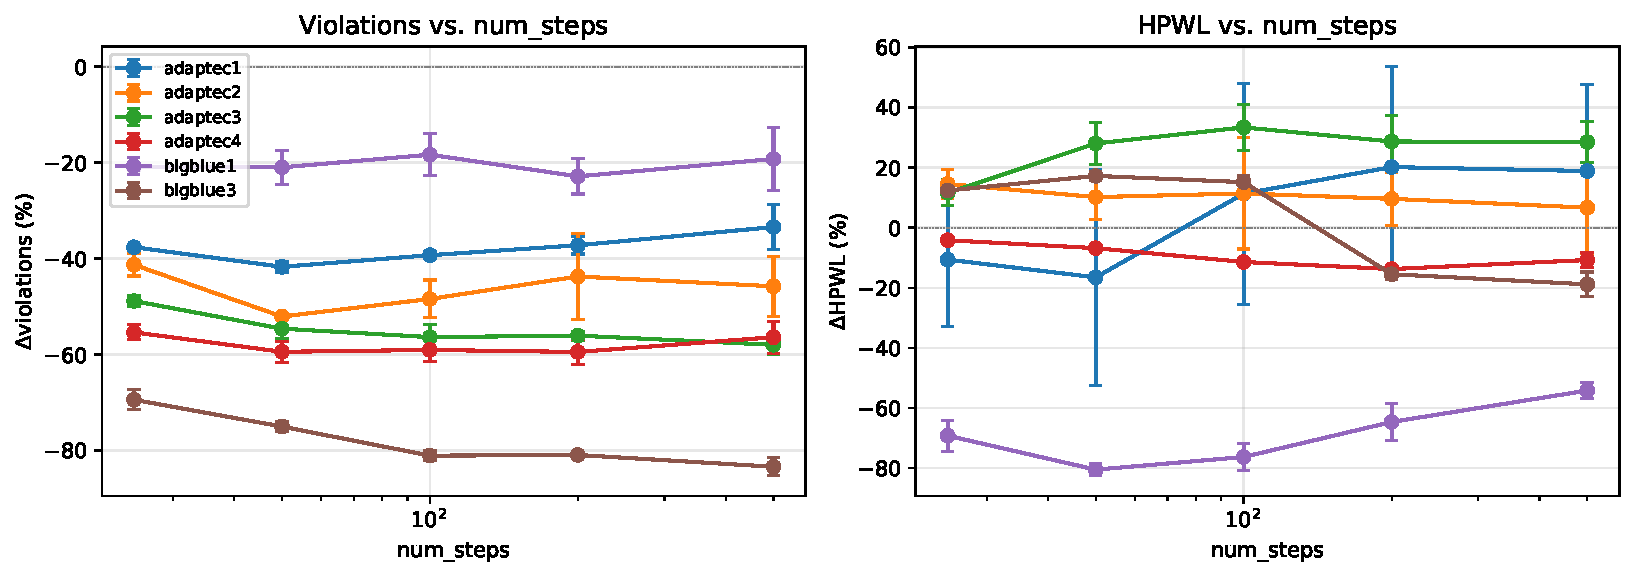
\includegraphics[width=0.85\linewidth]{figures/fig5_num_steps.pdf}
\caption{Number of repair steps ablation.}
\label{fig:supp-numsteps}
\end{figure}

\begin{figure}[h]
\centering
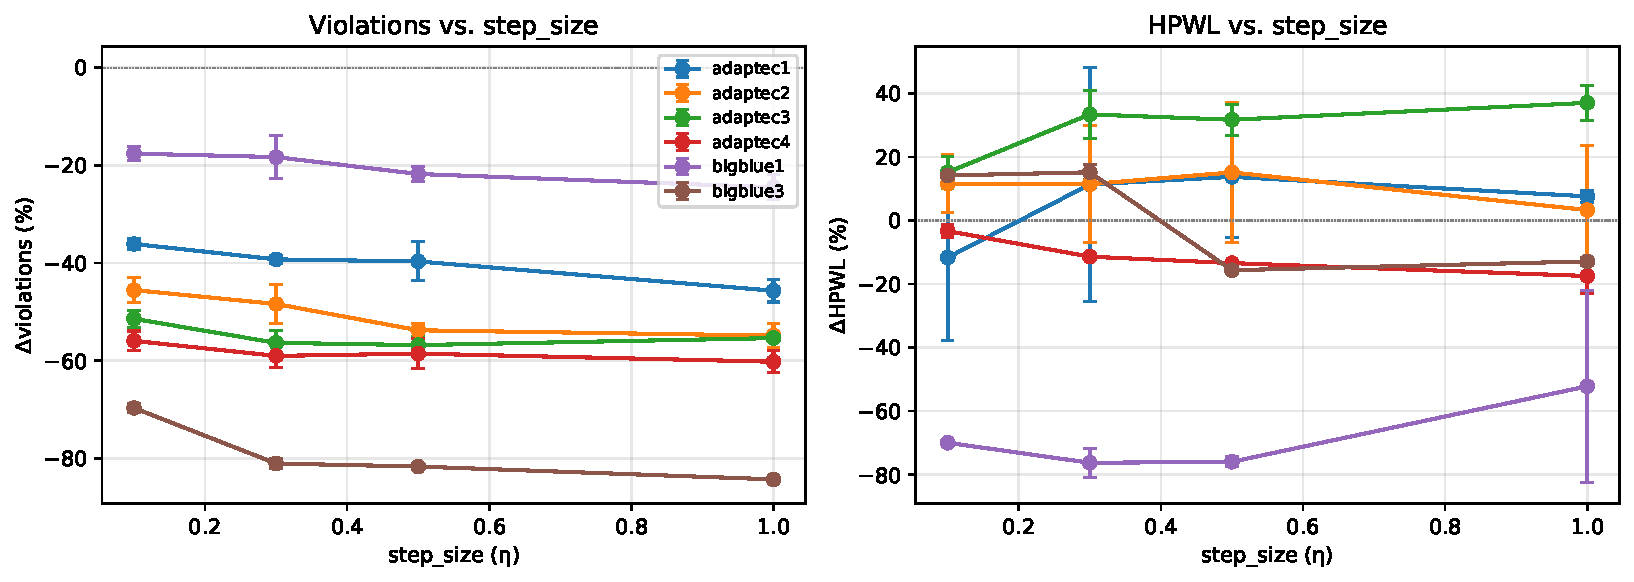
\includegraphics[width=0.85\linewidth]{figures/fig6_step_size.pdf}
\caption{Step size ablation.}
\label{fig:supp-stepsize}
\end{figure}

\begin{table}[h]
\centering
\begin{tabular}{lrrrr}
\toprule
Circuit & $\Delta$viol on & $\Delta$viol off & $\Delta$HPWL on & $\Delta$HPWL off \\
\midrule
adaptec1 & $-39.3$ & $-39.3$ & $+11.4$ & $+11.4$ \\
adaptec2 & $-48.4$ & $-48.4$ & $+11.4$ & $+11.4$ \\
adaptec3 & $-56.4$ & $-56.4$ & $+33.4$ & $+33.4$ \\
adaptec4 & $-59.0$ & $-59.0$ & $-11.4$ & $-11.4$ \\
bigblue1 & $-18.3$ & $-18.3$ & $-76.3$ & $-76.3$ \\
bigblue3 & $-81.1$ & $-81.1$ & $+15.2$ & $+15.2$ \\
\bottomrule
\end{tabular}
\caption{Selective vs.\ global repair.}
\label{tab:supp-selective}
\end{table}

\begin{figure}[h]
\centering
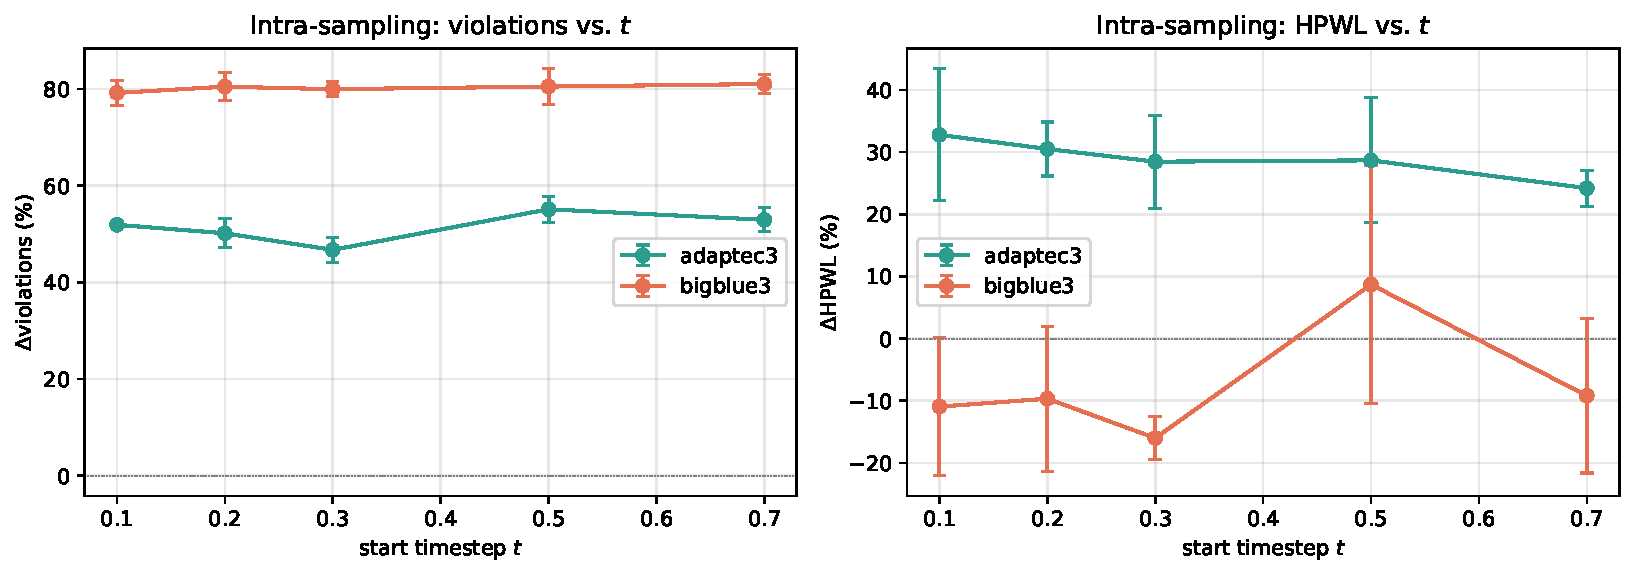
\includegraphics[width=0.85\linewidth]{figures/fig8_timestep_sweep.pdf}
\caption{Intra-sampling start timestep sweep.}
\label{fig:supp-timestep}
\end{figure}

\section{Memory profile of the diffusion backbone}
\label{sec:supp-mem}

We profile peak GPU memory of the ChipDiffusion backbone on the three
relevant circuits in three precisions; full per-precision table appears
in the main paper.  Two observations relevant to this supplement:

\begin{itemize}
\item Forward-step memory of the attention-GNN scales roughly with $N$
(macro count): $220$\,MB on adaptec2 ($N{=}566$), $1030$\,MB on bigblue4
($N{=}8170$), $2946$\,MB on bigblue2 ($N{=}23084$).  This is order-of-magnitude
linear, suggesting the bottleneck is the attention key/query/value matrices,
not the message passing.
\item Full-rollout memory (100 denoising steps) is approximately
$N$-times the forward step on small circuits but saturates near
$78$\,GB on the OOM circuits.  This is consistent with KV-cache-like
accumulation across the rollout that practical implementations of
flash-attention do not fully release between steps.
\end{itemize}

A natural future direction: replace the backbone's quadratic attention with
linear attention (e.g.\ Performer-style kernelized attention) on the macro-graph axis;
this would unblock bigblue2/4 evaluation.  We did not attempt this because
it would require backbone retraining.

Raw rows: \texttt{results/ispd2005/mem\_profile.json} (9 rows: 3 circuits
$\times$ 3 dtypes).

\section{Toy cross-domain experiment}
\label{sec:supp-toy2d}

We provide a toy 2D non-overlap experiment in
\texttt{scripts/toy\_2d\_experiment.py} that demonstrates the verifier-guided
repair operator outside the placement domain.  Setup: 30 random disks on a
unit canvas, sparse random graph, tiny per-disk denoiser trained on 1000
synthetic legal layouts.  Five methods compared: baseline (raw sample),
classifier-guidance (smooth softplus overlap penalty), RePaint with binary
mask, VSR-post, VSR-intra-soft.

This is a controlled cross-domain demonstration; we treat it as preliminary
support for the abstraction generalizing.  Note that toy denoiser quality
is sensitive to training set size; we recommend $\geq 1000$ training
layouts and $\geq 30,000$ training steps for a publication-quality run.

\section{Reproducibility}

All code, configs, checkpoints, and result JSONs are released. A single command reproduces all main-paper numbers:
\begin{verbatim}
  python scripts/run_all_experiments.py --config configs/paper_main.yaml
\end{verbatim}
on an A800 80GB GPU (or equivalent). The full sweep takes $\sim 20$ minutes.

\end{document}
